\documentclass[]{article}
\usepackage{lmodern}
\usepackage{amssymb,amsmath}
\usepackage{ifxetex,ifluatex}
\usepackage{fixltx2e} % provides \textsubscript
\ifnum 0\ifxetex 1\fi\ifluatex 1\fi=0 % if pdftex
  \usepackage[T1]{fontenc}
  \usepackage[utf8]{inputenc}
\else % if luatex or xelatex
  \ifxetex
    \usepackage{mathspec}
  \else
    \usepackage{fontspec}
  \fi
  \defaultfontfeatures{Ligatures=TeX,Scale=MatchLowercase}
\fi
% use upquote if available, for straight quotes in verbatim environments
\IfFileExists{upquote.sty}{\usepackage{upquote}}{}
% use microtype if available
\IfFileExists{microtype.sty}{%
\usepackage{microtype}
\UseMicrotypeSet[protrusion]{basicmath} % disable protrusion for tt fonts
}{}
\usepackage[margin=1in]{geometry}
\usepackage{hyperref}
\hypersetup{unicode=true,
            pdftitle={Data Mining Techniques Applied to Econometric Panel Data for FX Forecasting},
            pdfauthor={Charles Naylor},
            pdfborder={0 0 0},
            breaklinks=true}
\urlstyle{same}  % don't use monospace font for urls
\usepackage{color}
\usepackage{fancyvrb}
\newcommand{\VerbBar}{|}
\newcommand{\VERB}{\Verb[commandchars=\\\{\}]}
\DefineVerbatimEnvironment{Highlighting}{Verbatim}{commandchars=\\\{\}}
% Add ',fontsize=\small' for more characters per line
\usepackage{framed}
\definecolor{shadecolor}{RGB}{248,248,248}
\newenvironment{Shaded}{\begin{snugshade}}{\end{snugshade}}
\newcommand{\KeywordTok}[1]{\textcolor[rgb]{0.13,0.29,0.53}{\textbf{#1}}}
\newcommand{\DataTypeTok}[1]{\textcolor[rgb]{0.13,0.29,0.53}{#1}}
\newcommand{\DecValTok}[1]{\textcolor[rgb]{0.00,0.00,0.81}{#1}}
\newcommand{\BaseNTok}[1]{\textcolor[rgb]{0.00,0.00,0.81}{#1}}
\newcommand{\FloatTok}[1]{\textcolor[rgb]{0.00,0.00,0.81}{#1}}
\newcommand{\ConstantTok}[1]{\textcolor[rgb]{0.00,0.00,0.00}{#1}}
\newcommand{\CharTok}[1]{\textcolor[rgb]{0.31,0.60,0.02}{#1}}
\newcommand{\SpecialCharTok}[1]{\textcolor[rgb]{0.00,0.00,0.00}{#1}}
\newcommand{\StringTok}[1]{\textcolor[rgb]{0.31,0.60,0.02}{#1}}
\newcommand{\VerbatimStringTok}[1]{\textcolor[rgb]{0.31,0.60,0.02}{#1}}
\newcommand{\SpecialStringTok}[1]{\textcolor[rgb]{0.31,0.60,0.02}{#1}}
\newcommand{\ImportTok}[1]{#1}
\newcommand{\CommentTok}[1]{\textcolor[rgb]{0.56,0.35,0.01}{\textit{#1}}}
\newcommand{\DocumentationTok}[1]{\textcolor[rgb]{0.56,0.35,0.01}{\textbf{\textit{#1}}}}
\newcommand{\AnnotationTok}[1]{\textcolor[rgb]{0.56,0.35,0.01}{\textbf{\textit{#1}}}}
\newcommand{\CommentVarTok}[1]{\textcolor[rgb]{0.56,0.35,0.01}{\textbf{\textit{#1}}}}
\newcommand{\OtherTok}[1]{\textcolor[rgb]{0.56,0.35,0.01}{#1}}
\newcommand{\FunctionTok}[1]{\textcolor[rgb]{0.00,0.00,0.00}{#1}}
\newcommand{\VariableTok}[1]{\textcolor[rgb]{0.00,0.00,0.00}{#1}}
\newcommand{\ControlFlowTok}[1]{\textcolor[rgb]{0.13,0.29,0.53}{\textbf{#1}}}
\newcommand{\OperatorTok}[1]{\textcolor[rgb]{0.81,0.36,0.00}{\textbf{#1}}}
\newcommand{\BuiltInTok}[1]{#1}
\newcommand{\ExtensionTok}[1]{#1}
\newcommand{\PreprocessorTok}[1]{\textcolor[rgb]{0.56,0.35,0.01}{\textit{#1}}}
\newcommand{\AttributeTok}[1]{\textcolor[rgb]{0.77,0.63,0.00}{#1}}
\newcommand{\RegionMarkerTok}[1]{#1}
\newcommand{\InformationTok}[1]{\textcolor[rgb]{0.56,0.35,0.01}{\textbf{\textit{#1}}}}
\newcommand{\WarningTok}[1]{\textcolor[rgb]{0.56,0.35,0.01}{\textbf{\textit{#1}}}}
\newcommand{\AlertTok}[1]{\textcolor[rgb]{0.94,0.16,0.16}{#1}}
\newcommand{\ErrorTok}[1]{\textcolor[rgb]{0.64,0.00,0.00}{\textbf{#1}}}
\newcommand{\NormalTok}[1]{#1}
\usepackage{longtable,booktabs}
\usepackage{graphicx,grffile}
\makeatletter
\def\maxwidth{\ifdim\Gin@nat@width>\linewidth\linewidth\else\Gin@nat@width\fi}
\def\maxheight{\ifdim\Gin@nat@height>\textheight\textheight\else\Gin@nat@height\fi}
\makeatother
% Scale images if necessary, so that they will not overflow the page
% margins by default, and it is still possible to overwrite the defaults
% using explicit options in \includegraphics[width, height, ...]{}
\setkeys{Gin}{width=\maxwidth,height=\maxheight,keepaspectratio}
\IfFileExists{parskip.sty}{%
\usepackage{parskip}
}{% else
\setlength{\parindent}{0pt}
\setlength{\parskip}{6pt plus 2pt minus 1pt}
}
\setlength{\emergencystretch}{3em}  % prevent overfull lines
\providecommand{\tightlist}{%
  \setlength{\itemsep}{0pt}\setlength{\parskip}{0pt}}
\setcounter{secnumdepth}{0}
% Redefines (sub)paragraphs to behave more like sections
\ifx\paragraph\undefined\else
\let\oldparagraph\paragraph
\renewcommand{\paragraph}[1]{\oldparagraph{#1}\mbox{}}
\fi
\ifx\subparagraph\undefined\else
\let\oldsubparagraph\subparagraph
\renewcommand{\subparagraph}[1]{\oldsubparagraph{#1}\mbox{}}
\fi

%%% Use protect on footnotes to avoid problems with footnotes in titles
\let\rmarkdownfootnote\footnote%
\def\footnote{\protect\rmarkdownfootnote}

%%% Change title format to be more compact
\usepackage{titling}

% Create subtitle command for use in maketitle
\newcommand{\subtitle}[1]{
  \posttitle{
    \begin{center}\large#1\end{center}
    }
}

\setlength{\droptitle}{-2em}

  \title{Data Mining Techniques Applied to Econometric Panel Data for FX
Forecasting}
    \pretitle{\vspace{\droptitle}\centering\huge}
  \posttitle{\par}
    \author{Charles Naylor}
    \preauthor{\centering\large\emph}
  \postauthor{\par}
    \date{}
    \predate{}\postdate{}
  

\begin{document}
\maketitle

{
\setcounter{tocdepth}{2}
\tableofcontents
}
\section{Introduction}\label{introduction}

\subsection{Summary of Currency
Markets}\label{summary-of-currency-markets}

Macroeconomic forecasting is generally considered to be one of the
hardest challenges in finance. In comparison with forecasts on stocks or
bonds, currency (a.k.a ``foreign exchange'', or FX) price movements
react more purely to the flows of global trade and geopolitical risk,
because they have no intrinsic value. A currency's worth is quoted only
relative to other currencies.

\subsubsection{The Carry Trade}\label{the-carry-trade}

That said, there is still a basis for investing in currencies in that
any holding will earn interest, just like a savings account at a bank.
In the USA, the 3-month interest rate is about 2.3\%. In Turkey, it's
about 17\%. Other things being equal, an investor could borrow money in
American Dollars, then lend it out in Turkish Lira, and earn the
difference between these rates for a nearly 15\% annual return. This is
called the \textbf{carry trade}.

The carry trade is not riskless because the spot rate, i.e.~the number
of USD that a Turkish Lira can buy, is not fixed over this period. In
fact, undergraduate economics classes still teach that any profit
possible from this trade will be neatly ironed out due to spot price
movements, a phenomenon known as \textbf{Covered Interest Rate Parity}.
The persistance of the carry trade in the face of theory is a reminder
that economic models elide substantial frictions experienced in the real
world.

\subsubsection{Drivers of Returns}\label{drivers-of-returns}

In FX, that interest rate differential, the ``carry'', is relatively
stable but subject to punctuated equilibrium as new data comes to light.
In developed markets, this data primarily consists of central bank rate
decisions and the economic news that might affect those decisions. Price
movements, however, are the deterministic result of countless iterative,
interacting agents. While we may know many of these agents' motives, it
is not possible to aggregate their behavior with any accuracy, because
the actions of each agent are affected by those of all of the other
agents, and small measurement errors compound. For example, it is
impossible to tell the periodicity of market data without context. A
day's worth of price movements at 5-minute increments looks the same as
a year's worth of daily movements. The asset price measures the result
of a chaotic, nonlinear dynamical system: a scale-free
network\texttt{\textless{}insert\ reference\ to\ Barabasi\textgreater{}}.

\subsection{Motivation}\label{motivation}

Speculators in currencies try to pocket the carry while avoiding the
risk of major movements in currency prices. The strategy has been
likened to picking up nickels in front of a steamroller. Thus, in spite
of the difficulties inherent in forecasting currency movements, a
\emph{successful} speculator must have some idea of what those movements
will look like in the future.

There are many possible methods available to create these forecasts.
Professionally, econometric panel data (i.e.~the same set of economic
measurements repeated for multiple countries) has been plugged into a
Kalman Filter in order to capture the evolving relationship between
indicators and their currencies, while also recognizing that one
currency's movements will affect all other currencies. The Kalman filter
has the advantage of having a closed-form solution and being
well-adapted to testing in systems in which one expects to add new data
regularly. In its most basic form, the disadvantage is that a Kalman
filter requires careful tuning of the relationship between its output
variables, and of the covariance of evolution of its factor weightings.

Prior work has been done on the same data set as a case study of
generative Bayesian forecasting
techniques\texttt{\textless{}insert\ GP\ reference\textgreater{}}. The
study applied a Gaussian Process Regression to panel data for 11 of the
most traded world currencies. The result was a well-specified and
validated forecasting model whose error term was far larger than its
signal. This jibed with the results seen professionally using a Kalman
Filter, but thanks to posterior predictive checking the flaws are
glaringly obvious. Can this, or a similar forecast, be improved?

Work is being done at the University of Maryland into the application of
neural network reservoirs to chaotic
systems.\texttt{\textless{}insert\ Pathak\ reference\textgreater{}}
After surveying some simpler machine learning techniques, this project
will apply these techniques to the residuals of the Gaussian Process
regression, or in combination with some other regression on the panel
data.

\subsection{Goals}\label{goals}

\begin{itemize}
\tightlist
\item
  Run the panel data through a set of standard data mining techniques to
  provide a baseline.
\item
  Apply reservoir computing techniques to existing or new regressions.
\end{itemize}

\section{The Data}\label{the-data}

Data consists of the weekly currency returns, plus a raft of weekly
economic data.

\subsection{Y variables}\label{y-variables}

The endogenous, `Y' variable comprises weekly currency returns on 11
currencies for a ten-year period starting in 2007 and ending in 2017.

Weekly currency returns consist of the change in spot rate against the
US dollar, plus the carry, defined as the (time-adjusted) difference in
1 month forward rates between the local currency and the USD. Without
going into detail, the forward rates are a reasonable proxy for what a
professional speculator might expect to earn by placing trades using
currency derivatives.

It's important to note that our endogenous variable is
\emph{multivariate}. We cannot assume that different currencies have
returns that are independent of one another.

\begin{verbatim}
## Warning: Removed 22 rows containing missing values (geom_path).
\end{verbatim}

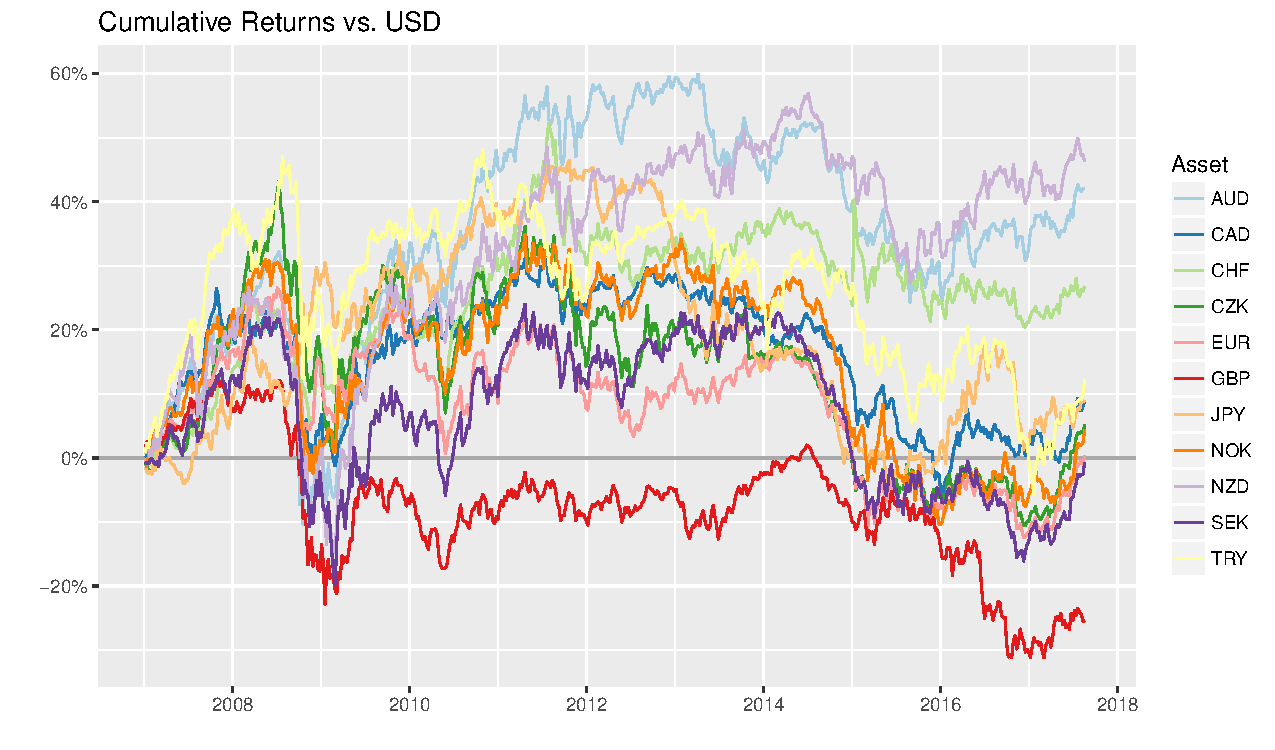
\includegraphics{Econometric_FX_Forecasting_files/figure-latex/graph_endos-1.pdf}

\subsection{X variables}\label{x-variables}

The exogenous, `X' variables consist of weekly data for the following:

\begin{longtable}[]{@{}ll@{}}
\toprule
Factor & Description\tabularnewline
\midrule
\endhead
Equity\_d8W & The 8 week change in the local equity index\tabularnewline
Spot\_d8W & The 8 week change in spot rates\tabularnewline
SwapRate2Y & The 2Y Swap Rate\tabularnewline
TwoYear\_d8W & The 8 week change in 2Y Swap rate\tabularnewline
YieldCurve & The spread between 10Y and 2Y Swaps\tabularnewline
\bottomrule
\end{longtable}

There is clear room for improvement if we were to fit a model that
permitted multiple time scales, such as a MIDAS
regression\texttt{\textless{}insert\ midas\ ref\textgreater{}}. It would
also be usual to include some sort of measure of liquidity and credit
conditions.

These variables have been scaled and normalized.

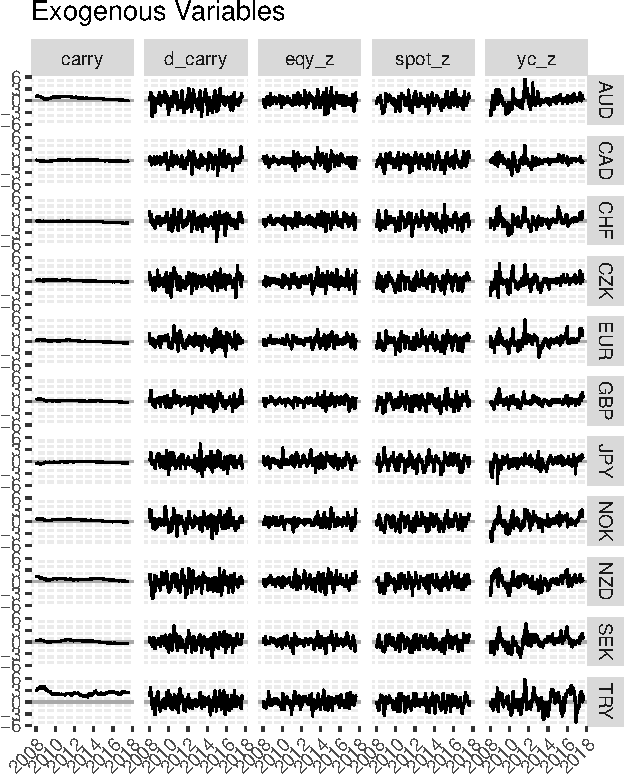
\includegraphics{Econometric_FX_Forecasting_files/figure-latex/graph_exogs-1.pdf}

Note that Carry is not a stochastic variable. It is, however, a rate,
and impacts asset returns consistently at that rate. It's also worth
noting the degree to which rate differentials have vanished since the
Credit Crisis of 2008.

\section{Models}\label{models}

\subsection{Classification}\label{classification}

\subsubsection{Introduction: Regime Switching
Models}\label{introduction-regime-switching-models}

There has been a substantial amount of work done in economic forecasting
in which time periods are split up into \emph{regimes}, periods in which
markets are expected to behave similarly given similar data. For
example, the markets in the run up to the bursting of the tech bubble in
2000, or the housing credit bubble in 2008, behaved substantially
differently to the markets just after those bubbles. The Kalman Filter
and Gaussian Process regression models attempt to account for changing
reactions to market conditions by fitting a continuously changing
regression to those conditions.

One alternative is a \textbf{Regime Switching Model}. Split the time
periods into several regimes, then run a separate regression for each
regime. The process is complicated by the fact what it can be extremely
difficult to tell at any given moment in which regime markets were
operating at any given time, even in hindsight.

One can attempt to determine these regimes by running various
classifiers and clustering algorithms against the exogenous and
endogenous data.

\subsubsection{Dissimilarity Matrixes}\label{dissimilarity-matrixes}

First it is necessary to compute a dissimilarity matrix between periods.
This calculates the distance between all of the values we have for each
week.

While fitting a global set of regimes, will give a more comprehensible
overview of the techniques, one set of regimes per country will be more
useful for forecasting, as the primary interest is in what happens when
there are differences between countries.

\paragraph{Global Regimes}\label{global-regimes}

Assume the market reactions to economic conditions are the same across
all countries.

\begin{Shaded}
\begin{Highlighting}[]
\CommentTok{# Organize data into per-row observation matrix}
\NormalTok{endo }\OperatorTok
\StringTok{  }\KeywordTok{gather}\NormalTok{(Asset, value, }\OperatorTok{-}\NormalTok{Date) }\OperatorTok
\StringTok{  }\KeywordTok{mutate}\NormalTok{(}\DataTypeTok{Exog=}\StringTok{"Endo"}\NormalTok{) }\OperatorTok
\StringTok{  }\KeywordTok{bind_rows}\NormalTok{(exogs) }\OperatorTok
\StringTok{  }\KeywordTok{filter}\NormalTok{(Date }\OperatorTok{>=}\KeywordTok{as.Date}\NormalTok{(}\StringTok{"2008-01-04"}\NormalTok{)) }\OperatorTok\StringTok{ }\CommentTok{#endo has more data than exog at the beginning}
\StringTok{  }\KeywordTok{filter}\NormalTok{(Date }\OperatorTok{<=}\KeywordTok{as.Date}\NormalTok{(}\StringTok{"2017-08-18"}\NormalTok{)) }\OperatorTok\StringTok{ }\CommentTok{#exog has more data than endo at the end}
\StringTok{  }\KeywordTok{unite}\NormalTok{(asset_exog, }\KeywordTok{c}\NormalTok{(}\StringTok{"Asset"}\NormalTok{, }\StringTok{"Exog"}\NormalTok{)) }\OperatorTok
\StringTok{  }\KeywordTok{spread}\NormalTok{(asset_exog, value) ->}
\StringTok{  }\NormalTok{all_obs_matrix}

\NormalTok{all_obs_matrix }\OperatorTok\StringTok{ }
\StringTok{  }\KeywordTok{select}\NormalTok{(}\OperatorTok{-}\NormalTok{Date) }\OperatorTok
\StringTok{  }\KeywordTok{daisy}\NormalTok{(}\DataTypeTok{metric=}\StringTok{"euclidean"}\NormalTok{) ->}
\StringTok{  }\NormalTok{global_dissimilarity}
\end{Highlighting}
\end{Shaded}

\paragraph{Principal Component
Analysis}\label{principal-component-analysis}

It will be hard to see what any of these clusters looks like, as the
feature space is high-dimensional. First, groupings of weeks were
examined using the first two principal components. These might form the
basis of later visualizations.

\begin{Shaded}
\begin{Highlighting}[]
\NormalTok{all_obs_matrix }\OperatorTok\StringTok{ }
\StringTok{  }\KeywordTok{select}\NormalTok{(}\OperatorTok{-}\NormalTok{Date) }\OperatorTok\StringTok{ }
\StringTok{  }\KeywordTok{prcomp}\NormalTok{() ->}\StringTok{ }
\StringTok{  }\NormalTok{global_pca}

\CommentTok{#Plot}
\NormalTok{(global_pca}\OperatorTok{$}\NormalTok{x }\OperatorTok\StringTok{ }\NormalTok{global_pca}\OperatorTok{$}\NormalTok{rotation[,}\DecValTok{1}\OperatorTok{:}\DecValTok{2}\NormalTok{]) }\OperatorTok
\StringTok{  }\KeywordTok{as_tibble}\NormalTok{() }\OperatorTok
\StringTok{  }\KeywordTok{bind_cols}\NormalTok{(all_obs_matrix }\OperatorTok\StringTok{ }
\StringTok{                }\KeywordTok{transmute}\NormalTok{(}\DataTypeTok{Year=}\KeywordTok{decimal_date}\NormalTok{(Date))) }\OperatorTok
\StringTok{  }\KeywordTok{ggplot}\NormalTok{(}\KeywordTok{aes}\NormalTok{(}\DataTypeTok{x=}\NormalTok{PC1,}\DataTypeTok{y=}\NormalTok{PC2, }\DataTypeTok{col=}\NormalTok{Year)) }\OperatorTok{+}
\StringTok{  }\KeywordTok{theme_bw}\NormalTok{() }\OperatorTok{+}
\StringTok{  }\KeywordTok{scale_color_gradient}\NormalTok{(}\DataTypeTok{low=}\StringTok{"red"}\NormalTok{,}\DataTypeTok{high=}\StringTok{"blue"}\NormalTok{)}\OperatorTok{+}
\StringTok{  }\KeywordTok{geom_point}\NormalTok{(}\DataTypeTok{alpha=}\FloatTok{0.25}\NormalTok{) }\OperatorTok{+}\StringTok{ }
\StringTok{  }\KeywordTok{ggtitle}\NormalTok{(}\StringTok{"First 2 Principal Components"}\NormalTok{)}
\end{Highlighting}
\end{Shaded}

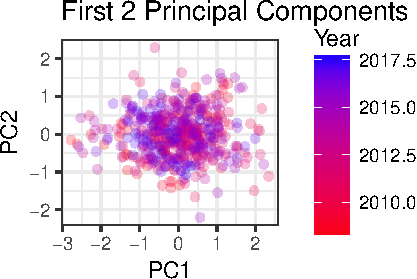
\includegraphics{Econometric_FX_Forecasting_files/figure-latex/pr_comp-1.pdf}
There is not much evidence of clear regime clusters here.

\paragraph{Per-Country Regimes}\label{per-country-regimes}

How similar are the regimes between countries? There may be an
identification issue as there's no guarantee that, e.g.~regime 1 in one
country will be encoded as regime 1 in another, even if they refer to
similar underlying clusters.

\subsubsection{Hierarchical Clustering}\label{hierarchical-clustering}

In hierarchical clustering, the observations are grouped by similarity
into progressively larger sections, creating a branching set of
categories. Given that the observer should expect relatively few broad
regimes of behavior in total, it will be necessary to cut these branches
early. Probably there should only be 2 or 3 regimes in total, but for
the purposes of validation, the cut was made at 5.

The identified cluster for each week can be seen below:

\begin{Shaded}
\begin{Highlighting}[]
\NormalTok{global_hclust <-}\StringTok{ }\KeywordTok{hclust}\NormalTok{(global_dissimilarity, }\DataTypeTok{method=}\StringTok{'complete'}\NormalTok{)}

\NormalTok{all_obs_matrix }\OperatorTok\StringTok{ }
\StringTok{  }\KeywordTok{select}\NormalTok{(Date) }\OperatorTok
\StringTok{  }\KeywordTok{mutate}\NormalTok{(}\DataTypeTok{Regime=}\KeywordTok{factor}\NormalTok{(}\KeywordTok{cutree}\NormalTok{(global_hclust, }\DataTypeTok{k=}\DecValTok{5}\NormalTok{)),}
         \DataTypeTok{Year=}\KeywordTok{factor}\NormalTok{(}\KeywordTok{year}\NormalTok{(Date)),}
         \DataTypeTok{Week=}\KeywordTok{week}\NormalTok{(Date)) }\OperatorTok
\StringTok{  }\KeywordTok{ggplot}\NormalTok{(}\KeywordTok{aes}\NormalTok{(}\DataTypeTok{x=}\NormalTok{Week, }\DataTypeTok{y=}\DecValTok{0}\NormalTok{, }\DataTypeTok{fill=}\NormalTok{Regime)) }\OperatorTok{+}
\StringTok{    }\KeywordTok{theme_pander}\NormalTok{() }\OperatorTok{+}
\StringTok{    }\KeywordTok{facet_grid}\NormalTok{(Year}\OperatorTok{~}\NormalTok{., }\DataTypeTok{switch=}\StringTok{"y"}\NormalTok{) }\OperatorTok{+}
\StringTok{    }\KeywordTok{geom_tile}\NormalTok{(}\DataTypeTok{color=}\StringTok{"white"}\NormalTok{) }\OperatorTok{+}\StringTok{ }
\StringTok{    }\KeywordTok{scale_fill_brewer}\NormalTok{(}\DataTypeTok{type=}\StringTok{"qual"}\NormalTok{,}\DataTypeTok{palette=}\StringTok{"Set1"}\NormalTok{) }\OperatorTok{+}
\StringTok{    }\KeywordTok{theme}\NormalTok{(}\DataTypeTok{strip.text.y =} \KeywordTok{element_text}\NormalTok{(}\DataTypeTok{angle=}\DecValTok{180}\NormalTok{),}
          \DataTypeTok{axis.text.y=}\KeywordTok{element_blank}\NormalTok{(), }
          \DataTypeTok{axis.ticks.y =} \KeywordTok{element_blank}\NormalTok{()) }\OperatorTok{+}\StringTok{ }\KeywordTok{ylab}\NormalTok{(}\StringTok{""}\NormalTok{) }\OperatorTok{+}
\StringTok{    }\KeywordTok{ggtitle}\NormalTok{(}\StringTok{"Hierarchical Clustering Global Regimes"}\NormalTok{)}
\end{Highlighting}
\end{Shaded}

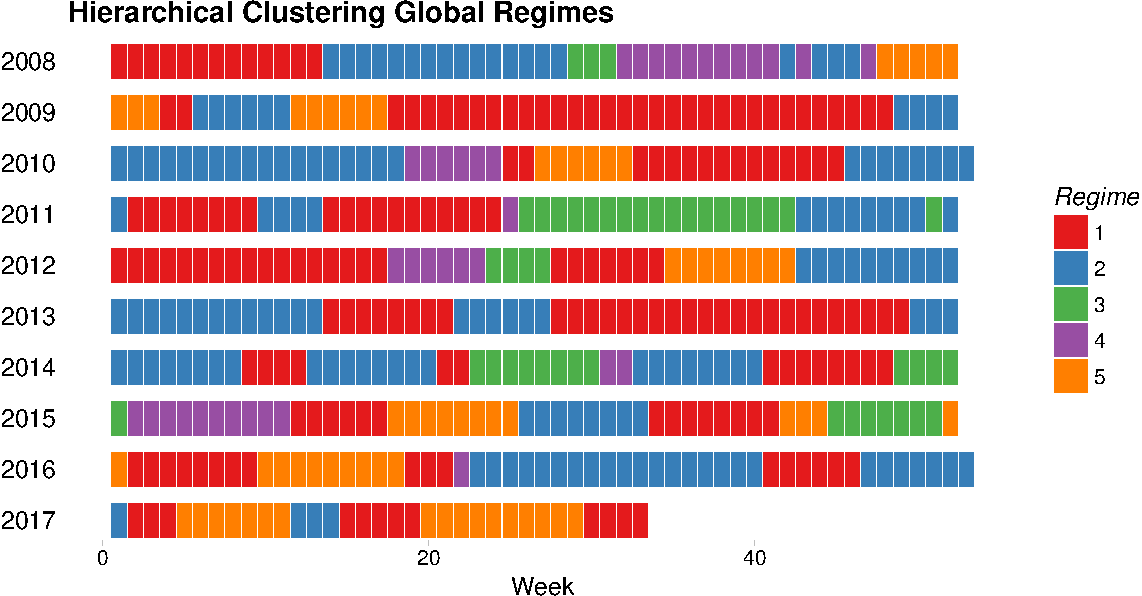
\includegraphics{Econometric_FX_Forecasting_files/figure-latex/hclust-1.pdf}
There are a lot of contiguous blocks, so the technique has clearly
identified something.

\paragraph{Per-country}\label{per-country}

How well does the technique work when applied to individual countries?

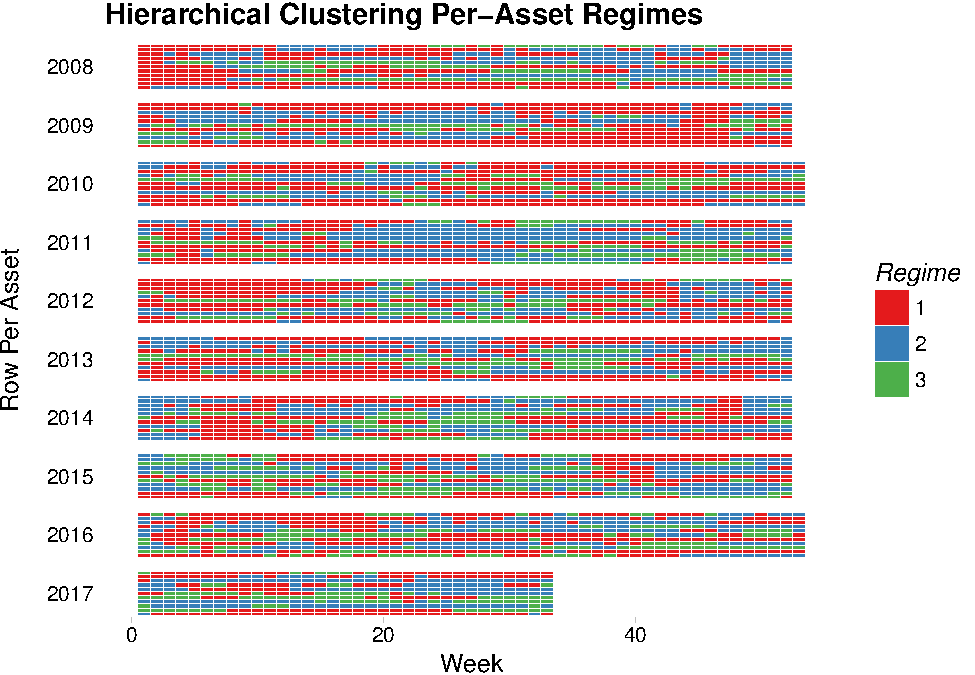
\includegraphics{Econometric_FX_Forecasting_files/figure-latex/per_asset_hclust-1.pdf}
There is still quite a lot of commonality between regimes. The least
similar currency is the Turkish Lira, on the bottom row. The British
Pound (middle row) enters a new regime 3 weeks \emph{before} the vote on
exiting the EU, in week 25 of 2016, which is evidence against the
validity of this technique.

\subsubsection{K-means Clustering}\label{k-means-clustering}

Unlike hierarchical clustering, K-means clustering looks at the data
holistically, and attempts to create groups of points around an
arbitrary number of centers. 5 centers were chosen to match the regimes
identified earlier.

\begin{Shaded}
\begin{Highlighting}[]
\NormalTok{global_kmeans <-}\StringTok{ }\KeywordTok{kmeans}\NormalTok{(all_obs_matrix }\OperatorTok\StringTok{ }\KeywordTok{select}\NormalTok{(}\OperatorTok{-}\NormalTok{Date),}
                        \DataTypeTok{centers=}\DecValTok{5}\NormalTok{)}

\NormalTok{all_obs_matrix }\OperatorTok\StringTok{ }
\StringTok{  }\KeywordTok{select}\NormalTok{(Date) }\OperatorTok
\StringTok{  }\KeywordTok{mutate}\NormalTok{(}\DataTypeTok{Regime=}\KeywordTok{factor}\NormalTok{(global_kmeans}\OperatorTok{$}\NormalTok{cluster),}
         \DataTypeTok{Year=}\KeywordTok{factor}\NormalTok{(}\KeywordTok{year}\NormalTok{(Date)),}
         \DataTypeTok{Week=}\KeywordTok{week}\NormalTok{(Date)) }\OperatorTok
\StringTok{  }\KeywordTok{ggplot}\NormalTok{(}\KeywordTok{aes}\NormalTok{(}\DataTypeTok{x=}\NormalTok{Week, }\DataTypeTok{y=}\DecValTok{0}\NormalTok{, }\DataTypeTok{fill=}\NormalTok{Regime)) }\OperatorTok{+}
\StringTok{    }\KeywordTok{theme_pander}\NormalTok{() }\OperatorTok{+}
\StringTok{    }\KeywordTok{facet_grid}\NormalTok{(Year}\OperatorTok{~}\NormalTok{., }\DataTypeTok{switch=}\StringTok{"y"}\NormalTok{) }\OperatorTok{+}
\StringTok{    }\KeywordTok{geom_tile}\NormalTok{(}\DataTypeTok{color=}\StringTok{"white"}\NormalTok{) }\OperatorTok{+}\StringTok{ }
\StringTok{    }\KeywordTok{scale_fill_brewer}\NormalTok{(}\DataTypeTok{type=}\StringTok{"qual"}\NormalTok{,}\DataTypeTok{palette=}\StringTok{"Set1"}\NormalTok{) }\OperatorTok{+}
\StringTok{    }\KeywordTok{theme}\NormalTok{(}\DataTypeTok{strip.text.y =} \KeywordTok{element_text}\NormalTok{(}\DataTypeTok{angle=}\DecValTok{180}\NormalTok{),}
          \DataTypeTok{axis.text.y=}\KeywordTok{element_blank}\NormalTok{(), }
          \DataTypeTok{axis.ticks.y =} \KeywordTok{element_blank}\NormalTok{()) }\OperatorTok{+}\StringTok{ }\KeywordTok{ylab}\NormalTok{(}\StringTok{""}\NormalTok{) }\OperatorTok{+}
\StringTok{    }\KeywordTok{ggtitle}\NormalTok{(}\StringTok{"Hierarchical Clustering Global Regimes"}\NormalTok{)}
\end{Highlighting}
\end{Shaded}

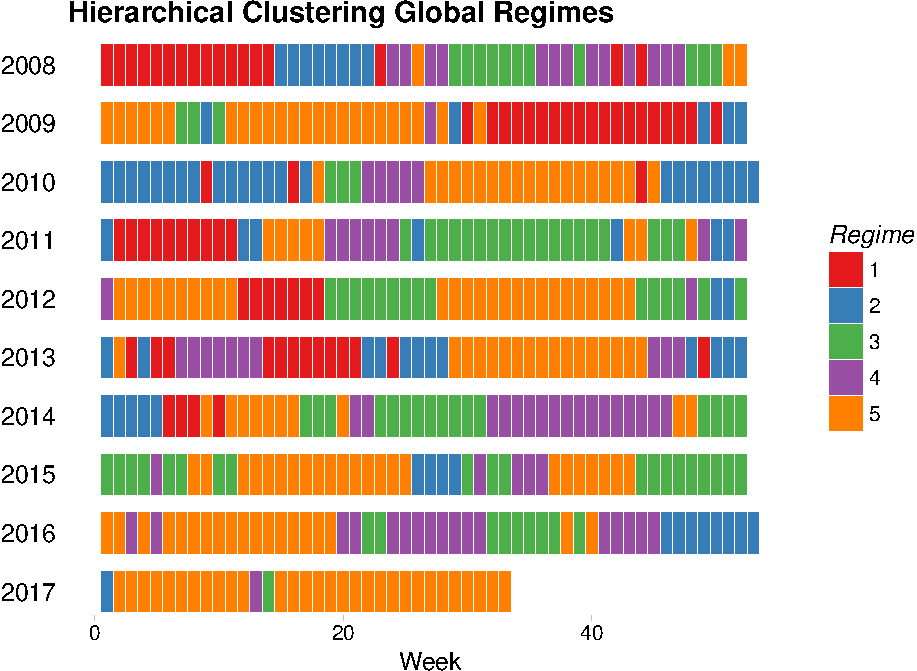
\includegraphics{Econometric_FX_Forecasting_files/figure-latex/global_kmean-1.pdf}

Although the Regime numbers are different, the pattern looks fairly
similar to the global regimes made using hierarchical clustering.

\section{Forecasting}\label{forecasting}

As with most other asset classes, currency returns have fat tails, and
the majority of an investor's profit (or loss) is typically made in a
small number of periods. Suprise economic news or geopolitical events
such as the British vote to leave the EU can cause the markets to
reassess appropriate price levels drastically. As a result, a person
discretizing returns so that a classifier can be applied directly would
be well-advised to distinguish between large moves and smaller ones. In
this analysis, discretization of the endogenous variable will be avoided
as much as possible.

One must also be careful when applying typical validation techniques,
particularly cross-validation, to time series. As the clustering
algorithms above clearly demonstrated, one cannot take samples of the
data that assume values will be independent of one another across time.
The ideal equivalent to leave-one-out cross-validation is simply to run
the algorithm every week with the data available for that week, keeping
a single period forecast each time. For the purposes of regressions
conducted with Support Vector Machines and Random Forests, however, the
data will be sliced into training and testing periods midway through the
time series.

To make things convenient, move the data out of tidy format, and match
up next week's returns to this week's forecasting data:

\begin{Shaded}
\begin{Highlighting}[]
\NormalTok{TRAINING_CUTOFF =}\StringTok{ }\KeywordTok{ymd}\NormalTok{(}\DecValTok{20121029}\NormalTok{)}
\CommentTok{#stack and combine lagged asset returns with exogenous variables}
\NormalTok{endo }\OperatorTok
\StringTok{  }\KeywordTok{mutate_at}\NormalTok{(}\KeywordTok{vars}\NormalTok{(}\OperatorTok{-}\NormalTok{Date),lead) }\OperatorTok\StringTok{ }\CommentTok{#dplyr parlance has moving endos one week back as a "lead".}
\StringTok{  }\KeywordTok{remove_missing}\NormalTok{() }\OperatorTok
\StringTok{  }\KeywordTok{gather}\NormalTok{(Asset, endo, }\OperatorTok{-}\NormalTok{Date) }\OperatorTok
\StringTok{  }\KeywordTok{inner_join}\NormalTok{(exogs, }\DataTypeTok{by=}\KeywordTok{c}\NormalTok{(}\StringTok{"Date"}\NormalTok{,}\StringTok{"Asset"}\NormalTok{)) }\OperatorTok\StringTok{ }
\StringTok{  }\KeywordTok{mutate}\NormalTok{(}\DataTypeTok{is_training=}\NormalTok{ Date}\OperatorTok{<}\NormalTok{TRAINING_CUTOFF) }\OperatorTok
\StringTok{  }\KeywordTok{spread}\NormalTok{(Exog, value) ->}
\StringTok{  }\NormalTok{forecast_data}
\end{Highlighting}
\end{Shaded}

\begin{verbatim}
## Warning: Removed 3 rows containing missing values.
\end{verbatim}

\begin{Shaded}
\begin{Highlighting}[]
\KeywordTok{glimpse}\NormalTok{(forecast_data)}
\end{Highlighting}
\end{Shaded}

\begin{verbatim}
## Observations: 5,522
## Variables: 10
## $ Date        <date> 2008-01-04, 2008-01-04, 2008-01-04, 2008-01-04, 2...
## $ Asset       <chr> "AUD", "CAD", "CHF", "CZK", "EUR", "GBP", "JPY", "...
## $ endo        <dbl> -0.0119246426, -0.0073437496, 0.0032708987, -0.021...
## $ is_training <lgl> TRUE, TRUE, TRUE, TRUE, TRUE, TRUE, TRUE, TRUE, TR...
## $ carry       <dbl> 0.9298046, 0.1128621, -0.1654536, 0.1353255, 0.197...
## $ constant    <dbl> 1, 1, 1, 1, 1, 1, 1, 1, 1, 1, 1, 1, 1, 1, 1, 1, 1,...
## $ d_carry     <dbl> -0.03776817, 0.16692213, 1.53078784, 0.20935335, 1...
## $ eqy_z       <dbl> -0.29407175, 0.45187138, 0.22751153, -0.13570337, ...
## $ spot_z      <dbl> -0.94082333, -1.60569442, -0.93559429, -1.20760013...
## $ yc_z        <dbl> -3.68560665, -0.24557129, -1.99447935, -3.34662631...
\end{verbatim}

\subsubsection{Support Vector Machines}\label{support-vector-machines}

Although Support Vector Machines (SVMs) are traditionally used for
classification, the technique can also be applied to regression.

The exogenous variables have already been standardized, so a SVM should
fit reasonably well out of the box. As we are forecasting at this point,
the endogenous variables (i.e.~the asset returns) will need to be lagged
by a week. Finally, there is the question of whether all currencies
should be expected to behave similarly given the same economic data. For
now, it will be assumed this is so.

Try an initial run without tuning:

\begin{Shaded}
\begin{Highlighting}[]
\NormalTok{forecast_data }\OperatorTok
\StringTok{  }\KeywordTok{filter}\NormalTok{(is_training) }\OperatorTok
\StringTok{  }\KeywordTok{select}\NormalTok{(}\OperatorTok{-}\NormalTok{constant, }\OperatorTok{-}\NormalTok{Date,}\OperatorTok{-}\NormalTok{Asset, }\OperatorTok{-}\NormalTok{is_training) }\OperatorTok\StringTok{ }\CommentTok{#a constant carries no information for a support vector machine, I believe}
\StringTok{  }\NormalTok{\{}\KeywordTok{svm}\NormalTok{(}\KeywordTok{as.formula}\NormalTok{(}\StringTok{"endo~."}\NormalTok{), }\DataTypeTok{data=}\NormalTok{., }\DataTypeTok{type=}\StringTok{"eps-regression"}\NormalTok{, }\DataTypeTok{kernel=}\StringTok{"radial"}\NormalTok{)\} ->}
\StringTok{  }\NormalTok{svm_base}
\KeywordTok{summary}\NormalTok{(svm_base)}
\end{Highlighting}
\end{Shaded}

\begin{verbatim}
## 
## Call:
## svm(formula = as.formula("endo~."), data = ., type = "eps-regression", 
##     kernel = "radial")
## 
## 
## Parameters:
##    SVM-Type:  eps-regression 
##  SVM-Kernel:  radial 
##        cost:  1 
##       gamma:  0.2 
##     epsilon:  0.1 
## 
## 
## Number of Support Vectors:  2504
\end{verbatim}

2500 support vectors suggests the regression may not be robust. How well
does it forecast returns for the remaining period?

\begin{Shaded}
\begin{Highlighting}[]
\NormalTok{forecast_data }\OperatorTok
\StringTok{  }\KeywordTok{filter}\NormalTok{(}\OperatorTok{!}\NormalTok{is_training) }\OperatorTok
\StringTok{  }\KeywordTok{select}\NormalTok{(}\OperatorTok{-}\NormalTok{constant, }\OperatorTok{-}\NormalTok{Date, }\OperatorTok{-}\NormalTok{Asset, }\OperatorTok{-}\NormalTok{is_training) }\OperatorTok
\StringTok{  }\NormalTok{\{}\KeywordTok{predict}\NormalTok{(svm_base, }\DataTypeTok{newdata =}\NormalTok{ .)\} ->}\StringTok{ }
\StringTok{  }\NormalTok{svm_base_hat}

\NormalTok{forecast_data }\OperatorTok
\StringTok{  }\KeywordTok{filter}\NormalTok{(}\OperatorTok{!}\NormalTok{is_training) }\OperatorTok
\StringTok{  }\KeywordTok{select}\NormalTok{(endo) }\OperatorTok\StringTok{ }
\StringTok{  }\KeywordTok{bind_cols}\NormalTok{(}\DataTypeTok{svm_base=}\NormalTok{svm_base_hat) }\OperatorTok
\StringTok{  }\KeywordTok{summarize}\NormalTok{(}\DataTypeTok{SSR=}\KeywordTok{sum}\NormalTok{((endo}\OperatorTok{-}\NormalTok{svm_base)}\OperatorTok{^}\DecValTok{2}\NormalTok{)) }\OperatorTok\StringTok{ }\KeywordTok{pull}\NormalTok{(SSR) }\OperatorTok\StringTok{ }\KeywordTok{print}\NormalTok{(}\DataTypeTok{digits=}\DecValTok{3}\NormalTok{)}
\end{Highlighting}
\end{Shaded}

\begin{verbatim}
## [1] 0.597
\end{verbatim}

It remains to be seen how good that SSR score is. Practitioners
typically have low expectations for goodness of fit and rely on various
performance metrics after applying an optimizer to the asset forecasts
to determine realistic investment decisions that could be based on the
results. Asset optimization is out of scope here, however.

\paragraph{Tuning the SVM}\label{tuning-the-svm}

The \texttt{e1071} package can perform a grid search on available
parameters and tune itself, however, the algorithm assumes that
cross-validation is an acceptable techniqe. The SVM will have to be
tuned manually.

What about a more parsimonious representation? The SVM algorithm permits
a regularization parameter, \texttt{cost}, which will penalize overly
complex models. It would also be sensible to try a polynomial kernel, as
asset returns, even normalized, are not expected to be linear with
respect to the economic data. Finally, it is likely this regression will
be noisy, so \(\gamma\) should be set low to reflect the high variance
in the data.

\begin{Shaded}
\begin{Highlighting}[]
\NormalTok{forecast_data }\OperatorTok
\StringTok{  }\KeywordTok{filter}\NormalTok{(is_training) }\OperatorTok
\StringTok{  }\KeywordTok{select}\NormalTok{(}\OperatorTok{-}\NormalTok{constant, }\OperatorTok{-}\NormalTok{Date,}\OperatorTok{-}\NormalTok{Asset, }\OperatorTok{-}\NormalTok{is_training) }\OperatorTok\StringTok{ }\CommentTok{#a constant carries no information for a support vector machine, I believe}
\StringTok{  }\NormalTok{\{}\KeywordTok{svm}\NormalTok{(}\KeywordTok{as.formula}\NormalTok{(}\StringTok{"endo~."}\NormalTok{), }\DataTypeTok{data=}\NormalTok{., }\DataTypeTok{type=}\StringTok{"eps-regression"}\NormalTok{, }\DataTypeTok{kernel=}\StringTok{"radial"}\NormalTok{, }\DataTypeTok{cost=}\DecValTok{1000}\NormalTok{)\} ->}
\StringTok{  }\NormalTok{svm_occam}
\KeywordTok{summary}\NormalTok{(svm_occam)}
\end{Highlighting}
\end{Shaded}

\begin{verbatim}
## 
## Call:
## svm(formula = as.formula("endo~."), data = ., type = "eps-regression", 
##     kernel = "radial", cost = 1000)
## 
## 
## Parameters:
##    SVM-Type:  eps-regression 
##  SVM-Kernel:  radial 
##        cost:  1000 
##       gamma:  0.2 
##     epsilon:  0.1 
## 
## 
## Number of Support Vectors:  2549
\end{verbatim}

The cost parameter actually increased the number of support vectors
found.

Fit a polynomial kernel:

\begin{Shaded}
\begin{Highlighting}[]
\NormalTok{forecast_data }\OperatorTok
\StringTok{  }\KeywordTok{filter}\NormalTok{(is_training) }\OperatorTok
\StringTok{  }\KeywordTok{select}\NormalTok{(}\OperatorTok{-}\NormalTok{constant, }\OperatorTok{-}\NormalTok{Date,}\OperatorTok{-}\NormalTok{Asset, }\OperatorTok{-}\NormalTok{is_training) }\OperatorTok\StringTok{ }\CommentTok{#a constant carries no information for a support vector machine, I believe}
\StringTok{  }\NormalTok{\{}\KeywordTok{svm}\NormalTok{(}\KeywordTok{as.formula}\NormalTok{(}\StringTok{"endo~."}\NormalTok{), }\DataTypeTok{data=}\NormalTok{., }\DataTypeTok{type=}\StringTok{"eps-regression"}\NormalTok{, }\DataTypeTok{kernel=}\StringTok{"polynomial"}\NormalTok{, }\DataTypeTok{coe0=}\DecValTok{0}\NormalTok{, }\DataTypeTok{d=}\DecValTok{3}\NormalTok{, }\DataTypeTok{cost=}\DecValTok{1000}\NormalTok{)\} ->}
\StringTok{  }\NormalTok{svm_poly}
\KeywordTok{summary}\NormalTok{(svm_poly)}
\end{Highlighting}
\end{Shaded}

\begin{verbatim}
## 
## Call:
## svm(formula = as.formula("endo~."), data = ., type = "eps-regression", 
##     kernel = "polynomial", coe0 = 0, d = 3, cost = 1000)
## 
## 
## Parameters:
##    SVM-Type:  eps-regression 
##  SVM-Kernel:  polynomial 
##        cost:  1000 
##      degree:  3 
##       gamma:  0.2 
##      coef.0:  0 
##     epsilon:  0.1 
## 
## 
## Number of Support Vectors:  2495
\end{verbatim}

This one failed to converge, so higher orders of polynomial are right
out.

Finally, set gamma low:

\begin{Shaded}
\begin{Highlighting}[]
\NormalTok{forecast_data }\OperatorTok
\StringTok{  }\KeywordTok{filter}\NormalTok{(is_training) }\OperatorTok
\StringTok{  }\KeywordTok{select}\NormalTok{(}\OperatorTok{-}\NormalTok{constant, }\OperatorTok{-}\NormalTok{Date,}\OperatorTok{-}\NormalTok{Asset, }\OperatorTok{-}\NormalTok{is_training) }\OperatorTok\StringTok{ }\CommentTok{#a constant carries no information for a support vector machine, I believe}
\StringTok{  }\NormalTok{\{}\KeywordTok{svm}\NormalTok{(}\KeywordTok{as.formula}\NormalTok{(}\StringTok{"endo~."}\NormalTok{), }\DataTypeTok{data=}\NormalTok{., }\DataTypeTok{type=}\StringTok{"eps-regression"}\NormalTok{, }\DataTypeTok{kernel=}\StringTok{"radial"}\NormalTok{, }\DataTypeTok{cost=}\DecValTok{1000}\NormalTok{, }\DataTypeTok{gamma=}\FloatTok{0.001}\NormalTok{)\} ->}
\StringTok{  }\NormalTok{svm_gamma}
\KeywordTok{summary}\NormalTok{(svm_gamma)}
\end{Highlighting}
\end{Shaded}

\begin{verbatim}
## 
## Call:
## svm(formula = as.formula("endo~."), data = ., type = "eps-regression", 
##     kernel = "radial", cost = 1000, gamma = 0.001)
## 
## 
## Parameters:
##    SVM-Type:  eps-regression 
##  SVM-Kernel:  radial 
##        cost:  1000 
##       gamma:  0.001 
##     epsilon:  0.1 
## 
## 
## Number of Support Vectors:  2514
\end{verbatim}

Compare the four models, using Mean Squared Error this time:

\begin{Shaded}
\begin{Highlighting}[]
\KeywordTok{list}\NormalTok{(}\DataTypeTok{base=}\NormalTok{svm_base, }\DataTypeTok{simple=}\NormalTok{svm_occam, }\DataTypeTok{poly=}\NormalTok{svm_poly, }\DataTypeTok{gamma=}\NormalTok{svm_gamma) }\OperatorTok
\StringTok{  }\KeywordTok{map_dfr}\NormalTok{(}\ControlFlowTok{function}\NormalTok{(model) \{}
\NormalTok{    forecast_data }\OperatorTok
\StringTok{      }\KeywordTok{filter}\NormalTok{(}\OperatorTok{!}\NormalTok{is_training) }\OperatorTok
\StringTok{      }\KeywordTok{select}\NormalTok{(}\OperatorTok{-}\NormalTok{constant, }\OperatorTok{-}\NormalTok{Date, }\OperatorTok{-}\NormalTok{Asset, }\OperatorTok{-}\NormalTok{is_training) }\OperatorTok
\StringTok{      }\NormalTok{\{}\KeywordTok{predict}\NormalTok{(model, }\DataTypeTok{newdata =}\NormalTok{ .)\} }\OperatorTok\StringTok{ }
\StringTok{      }\KeywordTok{bind_cols}\NormalTok{(}\DataTypeTok{hat=}\NormalTok{.,}
\NormalTok{                forecast_data }\OperatorTok\StringTok{ }
\StringTok{                  }\KeywordTok{filter}\NormalTok{(}\OperatorTok{!}\NormalTok{is_training) }\OperatorTok\StringTok{ }
\StringTok{                  }\KeywordTok{select}\NormalTok{(endo)) }\OperatorTok
\StringTok{      }\KeywordTok{summarize}\NormalTok{(}\DataTypeTok{MSE=}\DecValTok{10000}\OperatorTok{*}\KeywordTok{mean}\NormalTok{((endo}\OperatorTok{-}\NormalTok{hat)}\OperatorTok{^}\DecValTok{2}\NormalTok{)) }\OperatorTok\StringTok{ }
\StringTok{      }\KeywordTok{select}\NormalTok{(MSE) }
\NormalTok{  \}, }\DataTypeTok{.id=}\StringTok{"SVM"}\NormalTok{) }\OperatorTok
\StringTok{  }\NormalTok{knitr}\OperatorTok{::}\KeywordTok{kable}\NormalTok{(}\DataTypeTok{digits=}\DecValTok{3}\NormalTok{)}
\end{Highlighting}
\end{Shaded}

\begin{longtable}[]{@{}lr@{}}
\toprule
SVM & MSE\tabularnewline
\midrule
\endhead
base & 2.171\tabularnewline
simple & 11.369\tabularnewline
poly & 2.485\tabularnewline
gamma & 1.987\tabularnewline
\bottomrule
\end{longtable}

The model assuming higher noise did the best. Something very strange is
going on the the high-cost `simple' model, which wound up less simple
than the base.

It's notable for all of these that the number of support vectors is
close to the number of observations (around 90\%), and that high
penalties are not helping the model find an easier solution. SVMs are
probably the wrong approach for this forecasts this noisy.

\subsection{Random Forests}\label{random-forests}

Decision Trees (or Regression Trees, in the continuous case) divide
observations into sections according to their similarity, and relate
those sections to the endogenous variable. They are notoriously
unstable, however: a small change in data can result in a completely
different model. Random Forests attempt to address this instability by
taking random samples of the data and fitting separate sets of
Regression Trees to each set, then combining the results. In their raw
form, they must be used with caution as the random sampling will assume
observations are independent, when in fact they are correlated over
time. The \texttt{randomForest} function in R can also be set to return
a proximity measure, similar to the dissimilarity matrixes calculated
above for the classifiers. More on this later.

\begin{Shaded}
\begin{Highlighting}[]
\NormalTok{forecast_data }\OperatorTok
\StringTok{  }\KeywordTok{filter}\NormalTok{(is_training) }\OperatorTok
\StringTok{  }\KeywordTok{select}\NormalTok{(}\OperatorTok{-}\NormalTok{constant, }\OperatorTok{-}\NormalTok{Date, }\OperatorTok{-}\NormalTok{Asset, }\OperatorTok{-}\NormalTok{is_training) }\OperatorTok
\StringTok{  }\NormalTok{\{}\KeywordTok{randomForest}\NormalTok{(}\KeywordTok{as.formula}\NormalTok{(}\StringTok{"endo~."}\NormalTok{), }\DataTypeTok{data=}\NormalTok{.)\} ->}
\StringTok{  }\NormalTok{rf_base}

\KeywordTok{plot}\NormalTok{(rf_base)}
\end{Highlighting}
\end{Shaded}

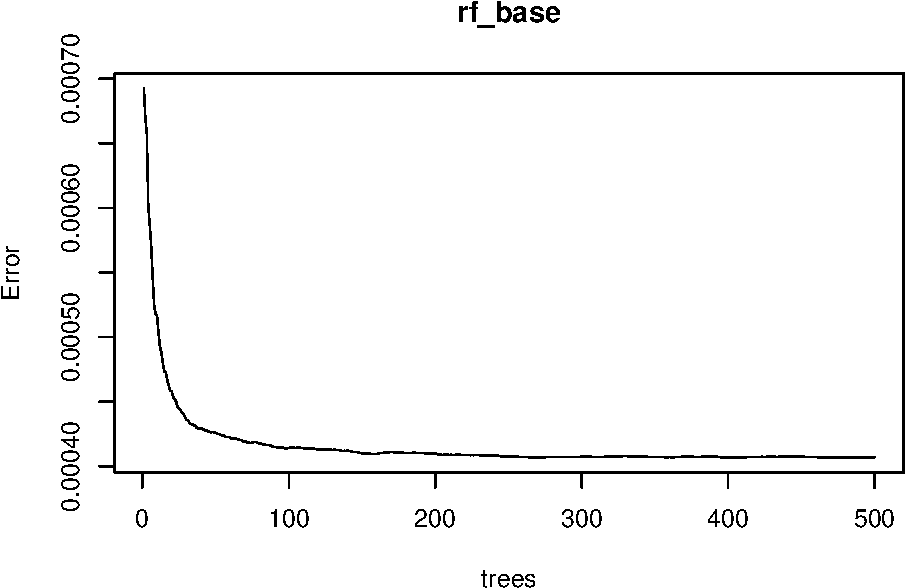
\includegraphics{Econometric_FX_Forecasting_files/figure-latex/rf-1.pdf}

There is not much gain from fitting more than about 25 trees.

As before, there should be relatively few nodes in the tree, reflecting
relatively few possible macroeconomic regimes for economies. How well
does the Random Forest regression do when \texttt{maxnodes} has been set
quite low?

\begin{Shaded}
\begin{Highlighting}[]
\NormalTok{forecast_data }\OperatorTok
\StringTok{  }\KeywordTok{filter}\NormalTok{(is_training) }\OperatorTok
\StringTok{  }\KeywordTok{select}\NormalTok{(}\OperatorTok{-}\NormalTok{constant, }\OperatorTok{-}\NormalTok{Date, }\OperatorTok{-}\NormalTok{Asset, }\OperatorTok{-}\NormalTok{is_training) }\OperatorTok
\StringTok{  }\NormalTok{\{}\KeywordTok{randomForest}\NormalTok{(}\KeywordTok{as.formula}\NormalTok{(}\StringTok{"endo~."}\NormalTok{), }\DataTypeTok{data=}\NormalTok{., }\DataTypeTok{maxnodes=}\DecValTok{20}\NormalTok{)\} ->}
\StringTok{  }\NormalTok{rf_fewnodes}

\KeywordTok{plot}\NormalTok{(rf_fewnodes)}
\end{Highlighting}
\end{Shaded}

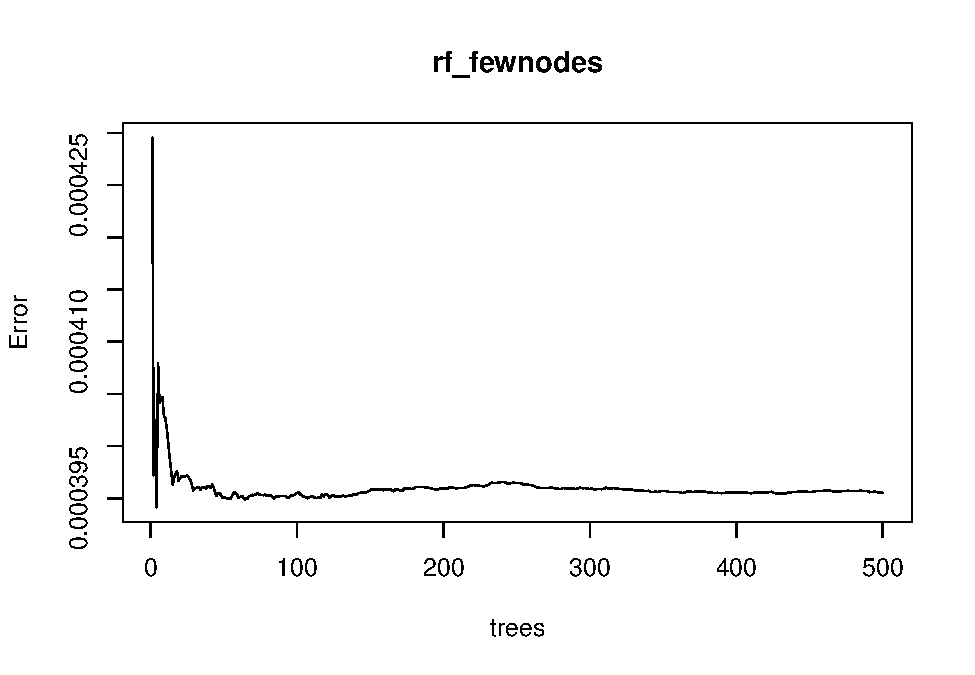
\includegraphics{Econometric_FX_Forecasting_files/figure-latex/rf_fewnodes-1.pdf}

That seems to have done just as well. Update the Mean Squared Error
table:

\begin{Shaded}
\begin{Highlighting}[]
\KeywordTok{list}\NormalTok{(}\DataTypeTok{svm_base=}\NormalTok{svm_base, }\DataTypeTok{svm_simple=}\NormalTok{svm_occam, }\DataTypeTok{svm_poly=}\NormalTok{svm_poly, }
     \DataTypeTok{svm_gamma=}\NormalTok{svm_gamma, }\DataTypeTok{rndForest=}\NormalTok{rf_base, }\DataTypeTok{rf_fewnodes=}\NormalTok{rf_fewnodes) }\OperatorTok
\StringTok{  }\KeywordTok{map_dfr}\NormalTok{(}\ControlFlowTok{function}\NormalTok{(model) \{}
\NormalTok{    forecast_data }\OperatorTok
\StringTok{      }\KeywordTok{filter}\NormalTok{(}\OperatorTok{!}\NormalTok{is_training) }\OperatorTok
\StringTok{      }\KeywordTok{select}\NormalTok{(}\OperatorTok{-}\NormalTok{constant, }\OperatorTok{-}\NormalTok{Date, }\OperatorTok{-}\NormalTok{Asset, }\OperatorTok{-}\NormalTok{is_training) }\OperatorTok
\StringTok{      }\NormalTok{\{}\KeywordTok{predict}\NormalTok{(model, }\DataTypeTok{newdata =}\NormalTok{ .)\} }\OperatorTok\StringTok{ }
\StringTok{      }\KeywordTok{bind_cols}\NormalTok{(}\DataTypeTok{hat=}\NormalTok{.,}
\NormalTok{                forecast_data }\OperatorTok\StringTok{ }
\StringTok{                  }\KeywordTok{filter}\NormalTok{(}\OperatorTok{!}\NormalTok{is_training) }\OperatorTok\StringTok{ }
\StringTok{                  }\KeywordTok{select}\NormalTok{(endo)) }\OperatorTok
\StringTok{      }\KeywordTok{summarize}\NormalTok{(}\DataTypeTok{MSE=}\DecValTok{10000}\OperatorTok{*}\KeywordTok{mean}\NormalTok{((endo}\OperatorTok{-}\NormalTok{hat)}\OperatorTok{^}\DecValTok{2}\NormalTok{)) }\OperatorTok\StringTok{ }
\StringTok{      }\KeywordTok{select}\NormalTok{(MSE) }
\NormalTok{  \}, }\DataTypeTok{.id=}\StringTok{"Model"}\NormalTok{) ->}
\StringTok{  }\NormalTok{MSE}
\NormalTok{  MSE }\OperatorTok
\StringTok{  }\KeywordTok{arrange}\NormalTok{(}\KeywordTok{desc}\NormalTok{(MSE)) }\OperatorTok
\StringTok{  }\NormalTok{knitr}\OperatorTok{::}\KeywordTok{kable}\NormalTok{(}\DataTypeTok{digits=}\DecValTok{3}\NormalTok{)}
\end{Highlighting}
\end{Shaded}

\begin{longtable}[]{@{}lr@{}}
\toprule
Model & MSE\tabularnewline
\midrule
\endhead
svm\_simple & 11.369\tabularnewline
svm\_poly & 2.485\tabularnewline
svm\_base & 2.171\tabularnewline
rndForest & 2.110\tabularnewline
svm\_gamma & 1.987\tabularnewline
rf\_fewnodes & 1.958\tabularnewline
\bottomrule
\end{longtable}

Fewer nodes made for a more robust model, but it is only marginally
better than the noise-tolerant SVM.

\subsection{Analogy Weighting}\label{analogy-weighting}

Jim Savage, currently chief Data Scientist at Lendable, Inc., invented
the technique of Analogy Weighting for his PhD thesis. His code is
available \href{https://github.com/khakieconomics/Thesis_work}{here}.
One runs a weighted linear regression on time series data using the
proximity matrix from a Random Forest regression for the weights. The
intuition is that similar periods in history ought to elicit similar
reactions to the data. Dr.~Savage used the data to forecast three
correlated economic time series. A key advantage of the analogy
weighting methodology is that the weights can be set such that the
regression is run on each data point without looking into the future.
This mimics the Kalman Filter workflow in that an investor need not fit
the entire model over again for each new data point. Alternately, one
can see an implementation of a Gaussian Process Regression on this same
data \href{https://charlesnaylor.github.io/gp_regression/}{here}. It was
necessary to fit the model over 500 times, which took considerable
processing power.

For an additional challenge, this forecast will take into account the
differences between countries, while fitting a single set of betas to
all. Outcomes will be modeled as arising from a multivariate normal
process to mimic the manner in which different countries' currencies
affect one another.

\begin{Shaded}
\begin{Highlighting}[]
\CommentTok{# Generate the proximity matrix once for each currency, then average}
\NormalTok{proximate <-}\StringTok{ }\ControlFlowTok{function}\NormalTok{(X) \{}
\NormalTok{    prox_mat <-}\StringTok{ }\KeywordTok{randomForest}\NormalTok{(endo}\OperatorTok{~}\NormalTok{carry}\OperatorTok{+}\NormalTok{d_carry}\OperatorTok{+}\NormalTok{eqy_z}\OperatorTok{+}\NormalTok{spot_z}\OperatorTok{+}\NormalTok{yc_z, }\DataTypeTok{data=}\NormalTok{X, }\DataTypeTok{proximity=}\OtherTok{TRUE}\NormalTok{)}\OperatorTok{$}\NormalTok{proximity}
    \KeywordTok{data.frame}\NormalTok{(}\DataTypeTok{Asset=}\NormalTok{X}\OperatorTok{$}\NormalTok{Asset, }\DataTypeTok{Date=}\NormalTok{X}\OperatorTok{$}\NormalTok{Date, prox_mat, }\DataTypeTok{stringsAsFactors =}\NormalTok{ F) }\OperatorTok
\StringTok{      }\KeywordTok{gather}\NormalTok{(x_Date,value,}\OperatorTok{-}\NormalTok{Asset,}\OperatorTok{-}\NormalTok{Date) }\OperatorTok
\StringTok{      }\KeywordTok{mutate}\NormalTok{(}\DataTypeTok{x_Date=}\NormalTok{X}\OperatorTok{$}\NormalTok{Date[}\KeywordTok{as.integer}\NormalTok{(}\KeywordTok{gsub}\NormalTok{(}\StringTok{"X"}\NormalTok{,}\StringTok{""}\NormalTok{,x_Date))]) }\CommentTok{#make sure the matrix stays lined up properly}
\NormalTok{\}}

\NormalTok{forecast_data }\OperatorTok
\StringTok{  }\KeywordTok{select}\NormalTok{(}\OperatorTok{-}\NormalTok{constant, }\OperatorTok{-}\NormalTok{is_training) }\OperatorTok\StringTok{ }
\StringTok{  }\KeywordTok{group_by}\NormalTok{(Asset) }\OperatorTok
\StringTok{  }\KeywordTok{do}\NormalTok{(}\KeywordTok{proximate}\NormalTok{(.)) }\OperatorTok
\StringTok{  }\KeywordTok{group_by}\NormalTok{(Date, x_Date) }\OperatorTok
\StringTok{  }\KeywordTok{summarize}\NormalTok{(}\DataTypeTok{value=}\KeywordTok{mean}\NormalTok{(value)) ->}
\StringTok{  }\NormalTok{proximity}

\NormalTok{proximity }\OperatorTok
\StringTok{  }\KeywordTok{mutate}\NormalTok{(}\DataTypeTok{value=}\KeywordTok{ifelse}\NormalTok{(x_Date}\OperatorTok{>=}\NormalTok{Date,}\DecValTok{0}\NormalTok{,value)) }\OperatorTok
\StringTok{  }\KeywordTok{ggplot}\NormalTok{(}\KeywordTok{aes}\NormalTok{(}\DataTypeTok{x=}\NormalTok{x_Date,}\DataTypeTok{y=}\NormalTok{Date,}\DataTypeTok{fill=}\NormalTok{value)) }\OperatorTok{+}
\StringTok{  }\KeywordTok{geom_tile}\NormalTok{() }\OperatorTok{+}\StringTok{ }\CommentTok{#I find myself using geom_tile a lot on this project}
\StringTok{  }\KeywordTok{scale_fill_gradient}\NormalTok{(}\DataTypeTok{low=}\StringTok{"white"}\NormalTok{, }\DataTypeTok{high=}\StringTok{"red"}\NormalTok{) }\OperatorTok{+}
\StringTok{  }\KeywordTok{coord_flip}\NormalTok{()}\OperatorTok{+}
\StringTok{  }\KeywordTok{ggtitle}\NormalTok{(}\StringTok{"Similarity between Dates"}\NormalTok{)}
\end{Highlighting}
\end{Shaded}

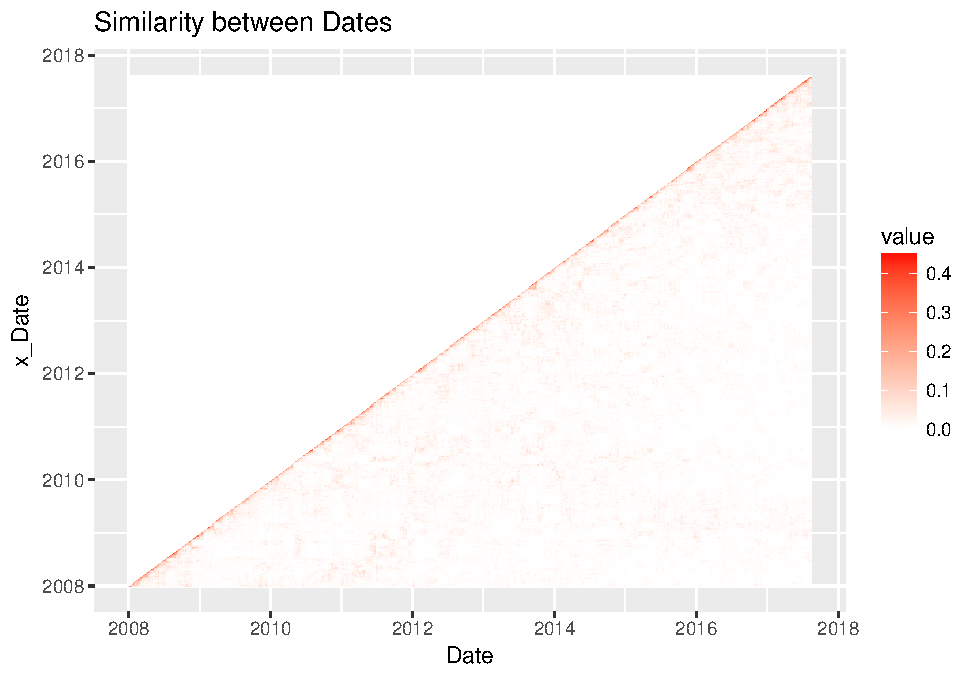
\includegraphics{Econometric_FX_Forecasting_files/figure-latex/proxmat-1.pdf}

Weightings will probably need to be normalized.

\subsubsection{Panel estimation of weighted
regressions}\label{panel-estimation-of-weighted-regressions}

The estimation of a multivariate endogenous variable is complex and best
expressed probabilistically using a generative model. Properly, fake
data should be generated with known parameters, and the model validated
by showing that it can recover those parameters. An example of the
validation workflow can be found can be found
\href{https://charlesnaylor.github.io/gp_regression/doc/Specifying_the_Model-Full_Model.html}{here}
for the Gaussian Process regression mentioned earlier.

The model will be fit using Stan, the current state of the art for
Bayesian generative models. Stan fits using Hamiltonian Monte Carlo, and
compiles directly to C for efficiency's sake, so the code in R will be
specified as a long string.

As a final input, the estimated covariance of the various currency
returns will be specified directly, for parsimony's sake. A production
system would typically estimate the joint volatility using a GARCH
model.

\begin{Shaded}
\begin{Highlighting}[]
\KeywordTok{suppressPackageStartupMessages}\NormalTok{(}\KeywordTok{library}\NormalTok{(rstan))}
\KeywordTok{rstan_options}\NormalTok{(}\DataTypeTok{auto_write =} \OtherTok{TRUE}\NormalTok{)}
\KeywordTok{options}\NormalTok{(}\DataTypeTok{mc.cores =}\NormalTok{ parallel}\OperatorTok{::}\KeywordTok{detectCores}\NormalTok{()) }\CommentTok{# MCMC techniques involve running multiple chains and ensuring they mixed well, an easily paralellized problem.}

\NormalTok{weighted_mvn_code <-}\StringTok{ "}
\StringTok{data \{}
\StringTok{  int<lower=0> A; // # of Assets}
\StringTok{  int<lower=0> T; // # of weeks (recall that the linear regression weighting permits testing on t+1 forecasts in a single step)}
\StringTok{  int<lower=0> J; // # of exogenous variables}
\StringTok{  int<lower=0> T_1; // #start of training period. We need some padding so the regression has enough periods to be useful }
\StringTok{  }
\StringTok{  row_vector[A] Y[T]; // asset returns}
\StringTok{  matrix[J,A] X[T]; //exogenous panel data}
\StringTok{  cov_matrix[A] y_cov[T]; // Covariance of asset returns}
\StringTok{  matrix[T,T] proxmat; //proximity matrix for weighting log-likelihood}
\StringTok{\}}
\StringTok{transformed data \{}
\StringTok{  int<lower=0> TL; //#training period length}
\StringTok{  matrix[A,A] L_y_cov[T];}
\StringTok{  TL = T - T_1;}
\StringTok{  for(t in 1:T) \{}
\StringTok{    L_y_cov[t] = cholesky_decompose(y_cov[t]); // Cholesky decompositions are more stably positive-definite than straight covariance matrices}
\StringTok{  \}}
\StringTok{\}}
\StringTok{parameters \{}
\StringTok{  matrix[TL, J] beta; // Shrunk betas across all assets. Could have been estimated as a state space model}
\StringTok{\}}
\StringTok{model \{}
\StringTok{  to_vector(beta) ~ normal(0, 1);}
\StringTok{  for(t in T_1:(T-1)) \{ //for each week in the data}
\StringTok{      for(i in 1:t) \{ //for each period prior to that week}
\StringTok{        target += proxmat[t,i] * multi_normal_cholesky_lpdf(Y[i]|beta[t-T_1+1]*X[i], L_y_cov[i]);}
\StringTok{      \}}
\StringTok{    \}}
\StringTok{\}}
\StringTok{generated quantities \{}
\StringTok{  //Generate forecasts so that we will have plenty of data to feed the neural net.}
\StringTok{  vector[A] y_hat[TL];}
\StringTok{  vector[TL] log_lik;}
\StringTok{  log_lik[1] = multi_normal_cholesky_lpdf(Y[T_1]|beta[T_1]*X[T_1], L_y_cov[T_1]);}
\StringTok{  for(t in (T_1+1):(T-1)) \{}
\StringTok{    log_lik[t-T_1+1] = multi_normal_cholesky_lpdf(Y[t]|beta[t-T_1+1]*X[t-T_1+1], L_y_cov[t-T_1+1]);}
\StringTok{    y_hat[t-T_1+1] = multi_normal_cholesky_rng(to_vector(beta[t-T_1]*X[t-T_1+1]), L_y_cov[t-T_1+1]);}
\StringTok{  \} }
\StringTok{\}}
\StringTok{"}

\NormalTok{weighted_mvn_model <-}\StringTok{ }\KeywordTok{stan_model}\NormalTok{(}\DataTypeTok{model_name=}\StringTok{"weighted_mvn"}\NormalTok{, }\DataTypeTok{model_code=}\NormalTok{weighted_mvn_code)}
\end{Highlighting}
\end{Shaded}

\begin{verbatim}
## In file included from /home/cnaylor/R/x86_64-pc-linux-gnu-library/3.2/BH/include/boost/config.hpp:39:0,
##                  from /home/cnaylor/R/x86_64-pc-linux-gnu-library/3.2/BH/include/boost/math/tools/config.hpp:13,
##                  from /home/cnaylor/R/x86_64-pc-linux-gnu-library/3.2/StanHeaders/include/stan/math/rev/core/var.hpp:7,
##                  from /home/cnaylor/R/x86_64-pc-linux-gnu-library/3.2/StanHeaders/include/stan/math/rev/core/gevv_vvv_vari.hpp:5,
##                  from /home/cnaylor/R/x86_64-pc-linux-gnu-library/3.2/StanHeaders/include/stan/math/rev/core.hpp:12,
##                  from /home/cnaylor/R/x86_64-pc-linux-gnu-library/3.2/StanHeaders/include/stan/math/rev/mat.hpp:4,
##                  from /home/cnaylor/R/x86_64-pc-linux-gnu-library/3.2/StanHeaders/include/stan/math.hpp:4,
##                  from /home/cnaylor/R/x86_64-pc-linux-gnu-library/3.2/StanHeaders/include/src/stan/model/model_header.hpp:4,
##                  from file1684ded9018.cpp:8:
## /home/cnaylor/R/x86_64-pc-linux-gnu-library/3.2/BH/include/boost/config/compiler/gcc.hpp:186:0: warning: "BOOST_NO_CXX11_RVALUE_REFERENCES" redefined
##  #  define BOOST_NO_CXX11_RVALUE_REFERENCES
##  ^
## <command-line>:0:0: note: this is the location of the previous definition
\end{verbatim}

Prepare the data in the format Stan expects. This was defined in the
\texttt{data} section above.

\paragraph{\texorpdfstring{\(\Sigma_y\)}{\textbackslash{}Sigma\_y}}\label{sigma_y}

Create exponentially weighted variance-covariance matrix. GARCH would be
better, but from prior experience makes little difference to weekly
currency returns.

\begin{Shaded}
\begin{Highlighting}[]
\NormalTok{FIRST_DATA_SET <-}\StringTok{ }\DecValTok{52} \CommentTok{#Start the forecast after we have at least 52 weeks of data}
\NormalTok{N1 <-}\StringTok{ }\KeywordTok{nrow}\NormalTok{(endo) }\OperatorTok{-}\StringTok{ }\DecValTok{1} \OperatorTok{-}\StringTok{ }\NormalTok{FIRST_DATA_SET}
\NormalTok{N2 <-}\StringTok{ }\DecValTok{0} \CommentTok{# # of extra periods}
\NormalTok{A <-}\StringTok{ }\KeywordTok{ncol}\NormalTok{(endo)}\OperatorTok{-}\DecValTok{1}

\NormalTok{y_cov <-}\StringTok{ }\KeywordTok{array}\NormalTok{(}\OtherTok{NA}\NormalTok{, }\DataTypeTok{dim=}\KeywordTok{c}\NormalTok{(N1}\OperatorTok{+}\NormalTok{N2, A, A))}

\NormalTok{lambda <-}\StringTok{ }\KeywordTok{exp}\NormalTok{(}\KeywordTok{log}\NormalTok{(}\FloatTok{0.5}\NormalTok{)}\OperatorTok{/}\DecValTok{52}\NormalTok{) }\CommentTok{# 1Y half-life exponential decay}
\NormalTok{wts <-}\StringTok{ }\NormalTok{lambda }\OperatorTok{^}\StringTok{ }\NormalTok{(}\KeywordTok{seq.int}\NormalTok{(}\DecValTok{0}\NormalTok{, y_offset}\OperatorTok{+}\NormalTok{N1}\OperatorTok{+}\NormalTok{N2))}
\ControlFlowTok{for}\NormalTok{(n }\ControlFlowTok{in} \DecValTok{1}\OperatorTok{:}\KeywordTok{nrow}\NormalTok{(y_cov)) \{}
\NormalTok{  ind <-}\StringTok{ }\KeywordTok{seq.int}\NormalTok{(FIRST_DATA_SET}\OperatorTok{+}\NormalTok{n}\OperatorTok{-}\DecValTok{1}\NormalTok{) }\CommentTok{#extra -1 in the index because we are lagging these an extra step}
\NormalTok{  y_cov[n,,] <-}\StringTok{ }\KeywordTok{cov.wt}\NormalTok{(endo[ind,}\OperatorTok{-}\DecValTok{1}\NormalTok{],}\KeywordTok{rev}\NormalTok{(wts[ind]), }\DataTypeTok{center=}\NormalTok{F)}\OperatorTok{$}\NormalTok{cov  }
\NormalTok{\}}
\end{Highlighting}
\end{Shaded}

Prepare the rest of the data

\begin{Shaded}
\begin{Highlighting}[]
\NormalTok{stan_data <-}\StringTok{ }\KeywordTok{list}\NormalTok{(}\DataTypeTok{A=}\KeywordTok{length}\NormalTok{(}\KeywordTok{unique}\NormalTok{(forecast_data}\OperatorTok{$}\NormalTok{Asset)),}
                  \DataTypeTok{T=}\KeywordTok{length}\NormalTok{(}\KeywordTok{unique}\NormalTok{(forecast_data}\OperatorTok{$}\NormalTok{Date)),}
                  \DataTypeTok{J=}\DecValTok{6}\NormalTok{,}\DataTypeTok{T_1=}\DecValTok{52}\NormalTok{,}
                  \DataTypeTok{Y=}\NormalTok{forecast_data }\OperatorTok\StringTok{ }
\StringTok{                    }\KeywordTok{select}\NormalTok{(Date, Asset, endo) }\OperatorTok\StringTok{ }
\StringTok{                    }\KeywordTok{spread}\NormalTok{(Asset, endo) }\OperatorTok
\StringTok{                    }\KeywordTok{select}\NormalTok{(}\OperatorTok{-}\NormalTok{Date),}
                  \DataTypeTok{X=}\NormalTok{forecast_data }\OperatorTok\StringTok{ }
\StringTok{                    }\KeywordTok{select}\NormalTok{(}\OperatorTok{-}\NormalTok{endo, }\OperatorTok{-}\NormalTok{is_training, }\OperatorTok{-}\NormalTok{Date) }\OperatorTok
\StringTok{                    }\KeywordTok{nest}\NormalTok{(}\OperatorTok{-}\NormalTok{Asset) }\OperatorTok
\StringTok{                    }\NormalTok{\{}\KeywordTok{abind}\NormalTok{(.}\OperatorTok{$}\NormalTok{data, }\DataTypeTok{along=}\DecValTok{3}\NormalTok{, }\DataTypeTok{new.names=}\NormalTok{.}\OperatorTok{$}\NormalTok{Asset)\},}
                  \DataTypeTok{y_cov=}\NormalTok{y_cov[}\DecValTok{3}\OperatorTok{:}\DecValTok{504}\NormalTok{,,],}
                  \DataTypeTok{proxmat=}\NormalTok{proximity }\OperatorTok\StringTok{ }
\StringTok{                    }\KeywordTok{ungroup}\NormalTok{() }\OperatorTok
\StringTok{                    }\KeywordTok{spread}\NormalTok{(x_Date, value) }\OperatorTok
\StringTok{                    }\KeywordTok{select}\NormalTok{(}\OperatorTok{-}\NormalTok{Date) }\OperatorTok\StringTok{ }
\StringTok{                    }\KeywordTok{as.matrix}\NormalTok{())}
\end{Highlighting}
\end{Shaded}

Run direct maximum likelihood optimization instead of Hamiltonian Monte
Carlo due to time constraints.

\begin{Shaded}
\begin{Highlighting}[]
\NormalTok{fit_weighted_mvn <-}\StringTok{ }\KeywordTok{optimizing}\NormalTok{(weighted_mvn_model, }\DataTypeTok{data=}\NormalTok{stan_data)}
\end{Highlighting}
\end{Shaded}

\begin{verbatim}
## Initial log joint probability = -4.215e+08
## Optimization terminated normally: 
##   Convergence detected: relative gradient magnitude is below tolerance
\end{verbatim}

Extract parameters

\begin{Shaded}
\begin{Highlighting}[]
\KeywordTok{matrix}\NormalTok{(fit_weighted_mvn}\OperatorTok{$}\NormalTok{par[}\KeywordTok{grep}\NormalTok{(}\StringTok{"beta"}\NormalTok{, }\KeywordTok{names}\NormalTok{(fit_weighted_mvn}\OperatorTok{$}\NormalTok{par))],}
       \KeywordTok{with}\NormalTok{(stan_data,T}\OperatorTok{-}\NormalTok{T_}\DecValTok{1}\NormalTok{), stan_data}\OperatorTok{$}\NormalTok{J, }\DataTypeTok{byrow=}\NormalTok{T, }\DataTypeTok{dimnames=}\KeywordTok{list}\NormalTok{(}\OtherTok{NULL}\NormalTok{, }\KeywordTok{unique}\NormalTok{(exogs}\OperatorTok{$}\NormalTok{Exog))) }\OperatorTok
\StringTok{  }\KeywordTok{as.data.frame}\NormalTok{() }\OperatorTok
\StringTok{  }\KeywordTok{mutate}\NormalTok{(}\DataTypeTok{Date=}\NormalTok{endo}\OperatorTok{$}\NormalTok{Date[stan_data}\OperatorTok{$}\NormalTok{T_}\DecValTok{1}\OperatorTok{:}\NormalTok{(stan_data}\OperatorTok{$}\NormalTok{T}\OperatorTok{-}\DecValTok{1}\NormalTok{)]) }\OperatorTok
\StringTok{  }\KeywordTok{gather}\NormalTok{(Exog,value,}\OperatorTok{-}\NormalTok{Date) ->}
\StringTok{  }\NormalTok{beta}

\NormalTok{beta }\OperatorTok\StringTok{ }
\StringTok{  }\KeywordTok{ggplot}\NormalTok{(}\KeywordTok{aes}\NormalTok{(}\DataTypeTok{x=}\NormalTok{Date, }\DataTypeTok{y=}\NormalTok{value, }\DataTypeTok{col=}\NormalTok{Exog)) }\OperatorTok{+}\StringTok{ }\KeywordTok{geom_line}\NormalTok{(}\DataTypeTok{alpha=}\FloatTok{0.6}\NormalTok{) }\OperatorTok{+}\StringTok{ }\KeywordTok{ggtitle}\NormalTok{(}\StringTok{"Betas over Time"}\NormalTok{) }\OperatorTok{+}\StringTok{ }\KeywordTok{scale_color_manual}\NormalTok{(}\DataTypeTok{values=}\NormalTok{exog_colors)}
\end{Highlighting}
\end{Shaded}

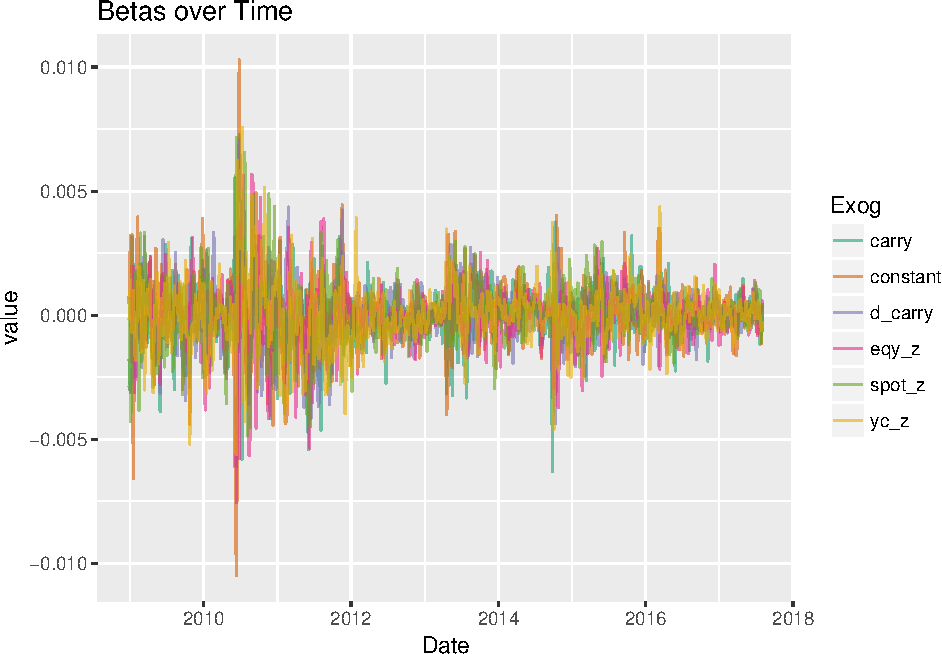
\includegraphics{Econometric_FX_Forecasting_files/figure-latex/unnamed-chunk-4-1.pdf}
The betas could be artificially induced to be more stable, as in a State
Space Model. The fact that they are not naturally so, and have such
small values, indicates that most of the variation in asset returns
cannot be explained by the weighted model.

How well did the model predict returns?

\begin{Shaded}
\begin{Highlighting}[]
\KeywordTok{matrix}\NormalTok{(fit_weighted_mvn}\OperatorTok{$}\NormalTok{par[}\KeywordTok{grep}\NormalTok{(}\StringTok{"y_hat"}\NormalTok{, }\KeywordTok{names}\NormalTok{(fit_weighted_mvn}\OperatorTok{$}\NormalTok{par))],}
       \KeywordTok{with}\NormalTok{(stan_data,T}\OperatorTok{-}\NormalTok{T_}\DecValTok{1}\NormalTok{), stan_data}\OperatorTok{$}\NormalTok{A, }\DataTypeTok{byrow=}\NormalTok{T, }\DataTypeTok{dimnames=}\KeywordTok{list}\NormalTok{(}\OtherTok{NULL}\NormalTok{, }\KeywordTok{colnames}\NormalTok{(endo)[}\OperatorTok{-}\DecValTok{1}\NormalTok{])) }\OperatorTok
\StringTok{  }\KeywordTok{as.data.frame}\NormalTok{() }\OperatorTok
\StringTok{  }\KeywordTok{mutate}\NormalTok{(}\DataTypeTok{Date=}\NormalTok{endo}\OperatorTok{$}\NormalTok{Date[stan_data}\OperatorTok{$}\NormalTok{T_}\DecValTok{1}\OperatorTok{:}\NormalTok{(stan_data}\OperatorTok{$}\NormalTok{T}\OperatorTok{-}\DecValTok{1}\NormalTok{)]) }\OperatorTok
\StringTok{  }\KeywordTok{gather}\NormalTok{(Asset,y_hat,}\OperatorTok{-}\NormalTok{Date) ->}
\StringTok{  }\NormalTok{y_hat}

\NormalTok{y_hat }\OperatorTok\StringTok{ }
\StringTok{  }\KeywordTok{drop_na}\NormalTok{() }\OperatorTok
\StringTok{  }\KeywordTok{inner_join}\NormalTok{(endo }\OperatorTok\StringTok{ }\KeywordTok{gather}\NormalTok{(Asset, value, }\OperatorTok{-}\NormalTok{Date), }\DataTypeTok{by=}\KeywordTok{c}\NormalTok{(}\StringTok{"Asset"}\NormalTok{,}\StringTok{"Date"}\NormalTok{)) }\OperatorTok\StringTok{ }
\StringTok{  }\KeywordTok{summarize}\NormalTok{(}\DataTypeTok{Model=}\StringTok{"analogy_mvn"}\NormalTok{, }\DataTypeTok{MSE=}\DecValTok{10000}\OperatorTok{*}\KeywordTok{mean}\NormalTok{((value}\OperatorTok{-}\NormalTok{y_hat)}\OperatorTok{^}\DecValTok{2}\NormalTok{)) }\OperatorTok\StringTok{ }
\StringTok{  }\KeywordTok{bind_rows}\NormalTok{(MSE) }\OperatorTok
\StringTok{  }\KeywordTok{arrange}\NormalTok{(}\KeywordTok{desc}\NormalTok{(MSE)) ->}
\StringTok{  }\NormalTok{MSE}
\NormalTok{MSE }\OperatorTok\StringTok{ }\NormalTok{knitr}\OperatorTok{::}\KeywordTok{kable}\NormalTok{(}\DataTypeTok{digits=}\DecValTok{3}\NormalTok{)}
\end{Highlighting}
\end{Shaded}

\begin{longtable}[]{@{}lr@{}}
\toprule
Model & MSE\tabularnewline
\midrule
\endhead
svm\_simple & 11.369\tabularnewline
analogy\_mvn & 6.570\tabularnewline
svm\_poly & 2.485\tabularnewline
svm\_base & 2.171\tabularnewline
rndForest & 2.110\tabularnewline
svm\_gamma & 1.987\tabularnewline
rf\_fewnodes & 1.958\tabularnewline
On its own, th & e analogy-weighted model is one of the poorest
options.\tabularnewline
\bottomrule
\end{longtable}

\subsection{Taming the Chaos}\label{taming-the-chaos}

\section{References}\label{references}


\end{document}
